\documentclass[11pt,a4paper]{report}
\usepackage[utf8x]{inputenc}
\usepackage[slovak,english]{babel}
\usepackage[IL2]{fontenc}
\usepackage{amsmath}
\usepackage{amsfonts}
\usepackage{amssymb}
\usepackage{makeidx}
\usepackage{graphicx}
\usepackage{lmodern}
\usepackage{subfig}
\usepackage[autostyle]{csquotes}
\usepackage{setspace}
\usepackage[left=3.5cm,right=2cm,top=2cm,bottom=2cm]{geometry}
\author{Bc. Michal Kohútek}
\title{Rozpoznávanie emocionálneho stavu používateľa pomocou inteligentných 
riadiacich systémov}

\graphicspath{ {./images/} }

\addto\captionsenglish{% Replace "english" with the language you use
  \renewcommand{\contentsname}%
    {Obsah}%
}


\usepackage{titlesec}
\titleformat{\chapter}[block]
{\normalfont\Large\bfseries}{\thechapter.}{1em}{\Large}
\titlespacing*{\chapter}{0pt}{-19pt}{19pt}


\titleformat{\section}[block]
{\normalfont\large\bfseries}{\thesection.}{1em}{\large}
\titlespacing*{\section}{0pt}{11pt}{19pt}

 \captionsetup[figure]{labelfont={bf},name={Obr.},labelsep=period}

\usepackage{scrpage2}
\ifoot[]{}
\cfoot[]{}
\ofoot[\pagemark]{\pagemark}


\begin{document}
\pagenumbering{gobble}
\begin{titlepage}
	
{\centering
{\bfseries\LARGE UNIVERZITA KONŠTANTÍNA FILOZOFA V NITRE \par}
{\bfseries\LARGE FAKULTA PRÍRODNÝCH VIED \par}
\vfill
{\bfseries\LARGE Informačné technológie\par}
\vspace{1cm}
{\bfseries\Large Vypracované otázky na štátnu skúšku\par}
\par}
\vfill


\Large{\noindent\textbf{Nitra 2018}\hfill\textbf{Bc. Michal Kohútek}}
\end{titlepage}

\tableofcontents

\chapter{Architektúra RISC a CISC}
\pagenumbering{arabic}
\setcounter{page}{2}
\pagestyle{scrplain}

\paragraph{Korpus:} \textit{Definícia pojmu procesor, rozdiel medzi architektúrami RISC a CISC, príklady spracovávania inštrukcií, využitie architektúry CISC v súčasnosti, výhody a nevýhody malého počtu inštrukcií. Pri uvádzaní rozdielov medzi jednotlivými architektúrami je potrebné, aby študent vedel rozlíšiť od seba nielen architektúru RISC a CISC, ale aby vedel popísať hlavne prečo vznikla nová architektúra RISC a čo ňou je možné dosiahnuť z hľadiska používania tzv. inštrukčných mixov.}

\section{CPU} Central Processing Unit, alebo procesor, interpretuje, vykonáva inštrukcie a spracúva dáta programu vo forme strojového kódu. V dnešnej dobe je zvyčajne realizovaný vo forme mikroprocesora. Historicky boli CPU implementované ako diskrétne komponenty a viacero malých integrovaných obvodov na jednej či viacerých doskách. Mikroprocesory sú CPU vyrábané zvyčajne na jednom integrovanom obvode. Zmenšenie veľkosti CPU prispieva k rýchlejšiemu prepínaniu, vďaka fyzickým faktorom, ako napríklad zníženej parazitickej kapacitancii. Hoci komplexnosť, veľkosť a výkon CPU sa od roku 1950 výrazne zmenili, základný dizajn a funkčnosť sa zachovali. Skoro všetky bežné CPU sa dajú pomerne presne popísať Von Neumannovou schémou.

\paragraph{Práca CPU} Základnou funkciou CPI je vykonávať sekvenciu uložených inštrukcií\footnote{program}. Vykonávané inštrukcie bývajú uložené v nejakej forme \textbf{počítačovej pamäti}. Skoro všetky CPU nasledujú fetch, decode a execute kroky v ich operácii, ktoré sa spolu nazývajú \textbf{inštrukčným cyklom.}. Po vykonaní inštrukcie sa celý proces zopakuje s nasledujúcou inštrukciou označenou inkrementovanou hodnotou v registri \textbf{program counter}. 
Pokiaľ sa vykonala inštrukcia \textbf{skoku}\footnote{jump}, program counter sa nastavi na cieľovú inštrukciu a vykonávanie programu prebieha ďalej normálne. Vo viac zložitých CPU sa môže vykonávať inštrukčný cyklus na viacerých inštrukciach súčasne. Niektoré inštrukcie (napríklad \textit{jump}) nemanipulujú dátami, ale zato upravujú program counter. Tým umožnujú praktiky, napr. cykly\footnote{for, while loop}, podmienené vykonávanie inštrukcií\footnote{if, switch-case} a existenciú funkcií.

\paragraph{Fetch} Prvý krok zaisťuje získanie inštrukcie z pamäte programu. Adresa inštrukcie je určená hodnotou v \textbf{PC} (program counter). Keď je inštrukcia získaná, PC je inkrementovaný dĺžkou inštrukcie tak, aby obsahoval adresu nasledujúcej inštrukcie. Keďže inštrukcie bývajú uložené v relatívne pomalých pamätiach (RAM, swapfile na disku), existuje riziko, že procesor bude na inštrukciu musieť čakať. Tento problém sa v moderných architektúrach rieši použitím cache a pipeline architektúr.

\paragraph{Decode} V tomto kroku sa inštrukcia konvertuje na signály, ktoré ovládajú ostatné časti CPU, za použitia \textbf{dekódera inštrukcií}\footnote{Instruction decoder}. Spôsob akým sa toto deje je definovaný architektúrou inštrukčnej sady\footnote{ISA, Instruction Set Architecture}. Zvyčajne jedna skupina bitov, zvaná opcode, označuje, ktorá operácia sa má vykonať, kým ostatné polia poskytujú dodatočné informácie dôležité pre operáciu, napr. operandy. Tieto operandy môžu byť konštatné hodnoty, alebo lokácie hodnoty, ktorá môźe byť buť register procesoru, alebo adresa pamäte. V niektorých dizajnoch CPU býva dekóder inštrukcií implementovaný ako nemeniteľný obvod. V iných sa na dekódovanie inštrukcií používa mikroprogram, ktorý môže byť prepísaný, čím sa dá upraviť spôsob, ako CPU dekóduje inštrukcie. Takto sa napríklad riešia zraniteľnosti, napr. Spectre a Meltdown.

\paragraph{Execute} Posledným krokom inštrukčného cyklu sa vykonávajú inštrukcie. V závislosti od architektúry CPU, toto môže byť spravené jednou akciou, alebo ich sekvenciou. Počas každej akcie sa rôzne časti CPU elektricky prepoja, aby mohli vykonať celú, či časť operácie v závislosti od tikotu hodín. Častokrát sa výsledny zapisujú do vnútorného registra CPU pre rýchly prístup z následujúcich inštrukcií. Pokiaľ sa k nim v skorej dobe nebude pristupovať, zapisujú sa do pomalšej, ale lacnejšej hlavnej pamäti. Napríklad ak sa má vykonať inštrukcia sčítania, vstupy do aritmeticko-logickej jednotky\footnote{ALU, Arithmetic Logic Unit} sú prepojené s párom operandov, výsledok sa objaví na výstupe, ktorý je pripojený na úložisko (register, alebo pamäť). Keď nastane tik hodín, výsledok sa presunie do úložiska a pokiaľ je výsledok väčší ako veľkosť výstupneho slova ALU, nastaví sa arithmetic overflow flag.

\paragraph{Štruktúra CPU} V CPU sú na pevno definované základné operácie, ktoré dokáže vykonávať, tzv. \textbf{inštrukčná sada}\footnote{instruction set}. Medzi takéto operácie patrí napríklad sčítanie, odčítanie, porovnanie dvoch čísel či skok do inej časti programu. Každá základná operácia je reprezentovaná kombináciou bitov, ktorá sa nazýva \textbf{opcode} strojového jazyka. Program v strojovom jazyku je zoskupenie inštrukcií v storjovom jazyku, ktoré CPU vykonáva. Matematické operácie pre každú inštrukciu sa vykonávajú kombinatorickým logickým obvodom, ktorý sa označuje ako Aritmeticko logická jednotka, alebo ALU. Základnými časťami procesora teda sú: 
\begin{itemize}
\item Aritmeticko-logická jednotka
\item Riadiaca jednotka\footnote{Control Unit}
\end{itemize}
Viac komplexné mikroprocesory súčasnosti obsahujú aj tzv. \textbf{jednotku prideľovania pamäte}, alebo \textbf{MMU}\footnote{Memory Management Unit}. Jednoduché procesory, napr. mikrokontroléry zvyčajne neobsahujú MMU.

\begin{figure}[ht]
        \centering
        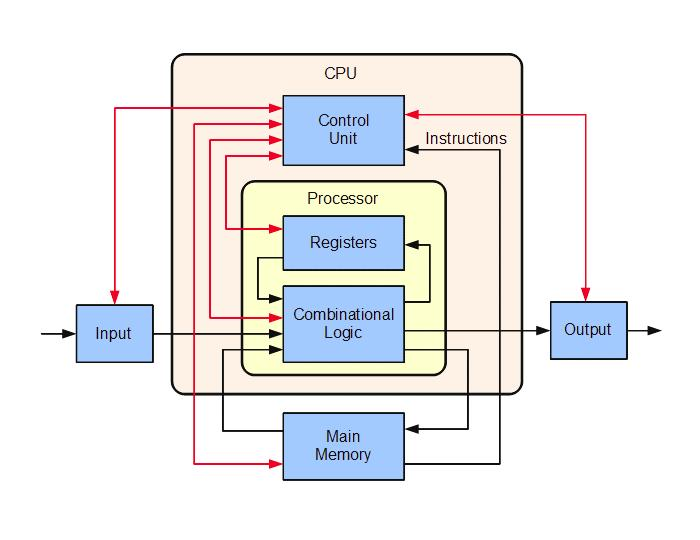
\includegraphics[scale=0.4]{images/ABasicComputer}
        \caption{Základná schéma CPU. Čierne čiary označujú tok dát, červené tok príkazov, šípky smer.}
        \label{CPU:}
\end{figure}
\newpage


\paragraph{ALU} Aritmeticko logická jednotka je kombinačný digitálny elektrický obvod, ktorý vykonáva aritmetické a bitové operácie na celočíselných binárnych číslach. Tento koncept navrhol John von Neumann v 1945 v správe o základoch nového počítača EDVAC. Na vstupe do ALU sú dáta, zvané operandy a kód operácie, ktorá má byť vykonaná. Na výstupe je výsledok vykonanej operácie. Vo viacerých dizajnoch má ALU aj stavové vstupy a výstupy, ktoré nesú informáciu o predchádzajúcej, alebo súčasnej operácie medzi ALU a externými stavovými registrami. 

\paragraph{CU} Ďalšou časťou von Neumannovej architektúry je riadiaca jednotka \footnote{Control Unit}. Je to komponent CPU, ktorý riadi činnosť procesora. Hovorí pamäti, ALU, a vstupno-výstupným zariadeniam ako majú reagovať na inštrukcie programu. Riadi operácie ostatných jednotiek poskytovaním časových a riadiacich signálov. CU riadi tok dát medzi CPU a ostatnými zariadeniami. Jednotlivé inštrukcie prechádzajú cez CU, ktorá ich dekóduje na niekoľko sekvenčných krokov, ktoré riadia a koordinujú vnútorné mechanizmi CPU pre správnu manipuláciu dát.

\paragraph{Registre} Registre  sú rýchlo dostupné oblasti prístupné procesoru. Zvyčajne obsahujú malé, no veľmi rýchle úložisko, hoci môžu mať aj iné, špecifické hardvérové funkcie. Pamäť v registri býva typicky adresovateľná mechanizmami oddelenými od hlavnej pamäte, no v istých prípadoch môžu mať pridelenú adresu pamäte. Skoro vo všetkých architektúrach sa dáta načítavajú z väčších pamätí do registrov, odkiaľ sa používajú v aritmetických operáciach. Výsledky sa bežne ukladajú do hlavnej pamäti. Poznáme rôzne kategórie registrov, líšiace sa účelom, použítím a množstvom bitov, ktoré môžu uchovávať.

\begin{itemize}
\item Používateľsky-prístupné registre 
      \begin{itemize}
      \item Dátové registre
      \item Adresové registre
      \item GPR \footnote{General-purpose registers} - môžu uchovávať dáta i adresy.
      \item Stavové registre
      \item Floating-point registre
      \item Registre konštánt - napr. 0, 1, $\pi$
      \item Vektorové registre - uchovávajú dáta pre SIMD\footnote{Single Instruction, Multiple Data}
      \item SPR\footnote{Special-purpose registers} - uchovávajú stav programu. Patrí sem program counter, status register.
      \item MTRR\footnote{Memory Type Range Registers} - sada registrov, ktoré poskytujú systému riadenie toho, ako sú prístupy CPU k pamäti cachované. 
      \end{itemize}
\item Vnútorné registre
\begin{itemize}
\item Register inštrukcií - drží informáciu o momentálne vykonávanej inštrukcií.
\item Registre oddelené od CPU súvisiace so získavaním informácie z RAM
\begin{itemize}
\item Memory buffer register (MBR)
\item Memory data register (MDR)
\item Memory address register (MAR)
\end{itemize}
\end{itemize}
\item Architektúrne registre
\end{itemize} 

\paragraph{Jednotka prideľovania pamäte} Memory Management Unit je komponent, skrz ktorý prechádzajú všetky pamäťové referencie a ktorý predovšetkým vykonáva preklad adries virtuálnej pamäte na fyzické adresy. Spravidla býva implementovaná ako súčasť CPU, avšak môže sa vyskytovať aj ako samostatný integrovaný obvod. MMU sa stará o manažment virtuálnej pamäte, tzn. riadi ochranu pamäte, riadenie cache, a v jednoduchších architektúrach aj tzv. "bank switching"\footnote{Technika ktorou sa v starších osem bitových počítačoch rozširovala pamäť nad rámec normálne adresovateľného priestoru. Bloky pamäte, ku ktorej bolo potrebné pristupovať len raz, napr. pri boote systému sa mohli vymeniť s prázdnou časťou operačnej pamäte.} Moderné MMU typicky delia adresný priestor na stránky, ktoré majú veľkosť v násobkoch 2, zvyčajne pár kilobytov, hoci môžu byť aj väčšie.
\begin{figure}[ht]
        \centering
        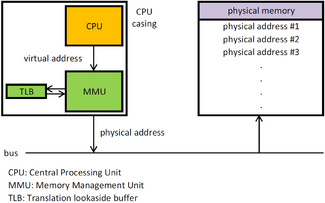
\includegraphics[scale=0.7]{images/MMU_principle_updated}
        \caption{Schéma práce MMU.}
        \label{MMU:}
\end{figure}

\section{Harvardská a Princetonská architektúra}


\section{RISC a CISC} \paragraph{ISA} Architektúra inštrukčnej sady je abstraktný model poitača. Realizácia ISA sa nazýva jej implementáciou. ISA definuje všetko čo musí programátor strojového jazyka vedieť na programovanie počítača. To, čo jednotlivé ISA definujú sa líši prípad od prípadu. Vo všeobecnosti definuje podporované dátové typy, stavy a ich sémantiky, inštrukčnú sadu a I/O model. ISA sa líši od mikroarchitektúry, čo je sada dizajnových techník použitých v konkrétnom procesore na implementáciu inštrukčnej sady. Procesory rôznych mikroarchitektúr môžu mať spoločnú inštrukčnú sadu. Napríklad procesory Intel Pentium a AMD Athlon implementujú takmer totožné verzie x86 inštrukčnej sady, hoci majú radikálne odlišný vnútorný dizajn. Dve hlavné kategórie ISA sú CISC\footnote{Complex Instruction Set Computer} a RISC \footnote{Reduced Instruction Set Computer}. Hoci sa jedná o protichodné koncepty, rozdiely medzi nimi sú však občas ťažko rozpoznateľné, keďze napríklad niektorí autori opisujú mikrokontroléry PIC ako RISC, iní zas ako CISC. Taktiež procesory x86, hoci sú CISC, mnoho z nich vnútorne používa mikrokód na konverziu komplexných inštrukcí na sekvenciu jednoduchších, ktoré potom vykoná. Hovorí sa preto, že hoci x86 \textbf{inštrukčná sada} je CISC, moderná x86 \textbf{architektúra} je RISC.

\tabcolsep=0.10cm
\begin{center}
\begin{tabular}{ | c | c | }
 \hline
 CISC  & RISC \\ 
 \hline
 \hline
 Dôraz na hardvér & Dôraz na softvér\\
 \hline
  Aj viac-taktové komplexné inštrukcie & Len jedno-taktové redukované inštrukcie \\ 
 \hline
 "LOAD" a "STORE" vstavané v inštrukciách & "LOAD" a "STORE" ako nezávislé inštrukcie \\ 
 \hline
 Menšia veľkosť kódu, viac cyklov za sekundu & Menej cyklov za sekundu, väčšia veľkost kódu \\ 
 \hline
 Tranzistory ukladajú komplexné inštrukcie & Viac tranzistorov v pamäťových registroch \\ 
 \hline
\end{tabular}
\end{center}

\paragraph{CISC} Starší z typov. Jednotlivé inštrukcie sú schopné vykonávať viacero nízko-úrovnňových operácií\footnote{Napr. načítanie z pamäte, aritmetické operácie, či uloženie do pamäti.}, alebo viackrokových operácií, či adresových módov počas jednej inštrukcie. Keďže sa tento názov začal používať retroaktívne po nástupe RISC procesorov, slúži ako kolektívny názov pre všetko, čo nie je RISC, či už sa jedná o komplexné sálové počítače, po najjednoduchśie mikrokontroléry, kde ukladanie a načítanie z pamäti nie sú oddelené od aritmetických inštrukcií. Z tohto dôvodu môže byť paradoxne moderný RISC procesor výrazne komplexnejší ako napríklad moderný CISC mikrokontroler, obzvlášť z hľadiska komplexnosti elektrických obvodov, ale aj počtom inštrukcií či ich zložitosti. Jediná typicky odlišujúca charakteristika je, že väčšina RISC dizajnov používa jednotnú inštrukčnú dĺžku pre skoro všetky svoje inštrukcie a striktne oddeluje inštrukcie load/store od ostatných.

\subparagraph{Výhody CISC}Predtým, než sa uplatnila dizajnová filozofia RISC, mnoho počítačových architektov sa snažilo zmenšiť takzvanú "sémantickú priepasť", tzn. navrnúť inštrukćné sady priamo podporujúce programovacie konštrukty vyššej úrovne, napr. volania procedúr, cykly a komplexné adresné režimy, umožňujúce dátovú štruktúru a prístupy k poliam skombinovať do jednotlivých inštrukcií. Inštrukcie sú typicky vysoko kódované, aby sa navýšila hustota kódu. Takáto kompaktnosť vedie k menším programom a menšiemu počtu prístupov do hlavnej (pomalej) pamäti, čo v dobe vzniku\footnote{60. roky 20. storočia} viedlo k veľkému šetreniu na cene pamäte a úložiska, a aj rýchlosti výpočtov. Taktiež to viedlo k lepšej produktivite programátorov aj v assembly, keďže vysoko úrovňové jazyky ako Fortran a Algol neboli vždy dostupné, alebo vhodné.

\subparagraph{Pridávanie inštrukcí} V 70. rokoch sa predpokladalo, že pridanie ďalších inštrukcií by mohlo navýšiť výpočtový výkon. Kompilátory boli aktualizované, aby využili tieto inštrukcie a takýto prístup sa používa v procesoroch dodnes, keďže prístupy do hlavnej operačnej pamäte sú stále niekoľko rádovo pomalšie ako činnosť jadra CPU.

\subparagraph{Nevýhody dizajnu} Kým úmyslom navyšovania počtu inštruikcí bolo zvýšiť výkon a umožniť vysoko úrovňovým jazykovým konštruktom vyjadrenie menším počtom inštrukcií, nie vždy sa to takto darilo. Architekti občas predizajnovali inštrukcie strojového jazyka, zahrňujúc funkcie, ktoré nemohli byť efektívne implementované na hardvéri. 


\paragraph{RISC} Táto architektúra umožnuje počítačom potrebovať menej cyklov na inštrukciu, ako porovnateľný CISC. Koncept RISC sa datuje do 80. rokov minulého storočia. O jeho popularizáciu sa zaslúžili najmä dva projekty zo Standfordskej univerzity a Univesity of California, Berkeley. Standfordská MIPS architektúra sa neskôr úspešne skomercializovala, kým architektúra vyvinutá v Berkeley, RISC, dala názov celému konceptu a ujala sa ako SPARC. Rôzne varianty RISC dizajnu zahrňujú  ARC, Alpha, Am29000, ARM, Atmel AVR, Blackfin, i860, i960, M88000, MIPS, PA-RISC, Power ISA (including PowerPC), RISC-V, SuperH, and SPARC.

\subparagraph{} Hoci sa podobné koncepty a implementácie objavovali už skôr, napr. CDC 6600 navrhnuté Seymourom Crayom v 1964, Michael J. Flynn považuje za prvý RISC systém IBM 801. Do vývoja RISC sa dapojila aj DARPA skz svoj VLSI\footnote{Very-Large-Scale Integration} program. Berkeley RISC bol navrhnutý tak, aby získal náskok vo výkone použitím pipeliningu a agresívnym používaním techniky register windowing. V tradičnom CPU je len malý počet registrov a program k nim môže kedykoľvek pristupovať. V CPU s oknami registrov je obrovský počet registrov, ale programy môžu využívať naraz len malý počet z nich. Program, ktorý sa limituje na osem registrov na procedúru môže vykonávať veľmi rýchle volania. Volanie jednoducho "posunie" okno nadol o osem, k sade registrov, ktoré procedúra vyoužíva a pri návrate posunie okno späť. RISC-I procesor, vyvinutý v 1982 pozostával z 44 420 tranzistorov (oproti cca 100 000 v CISC procesoroch tej doby), mal len 32 inštrukcií, no vo výkone prekonal všetky ostatné jednočipové dizajny. Neskôr ho predčili procesorom RISC-II s 40 760 tranzistormi a 39 inštrukciami, ktorý bol 3x rýchlejší ako RISC-I.

\subparagraph{} V 2010 sa objavila nová, open source ISA RISC-V, vyvinutá v Berkeley pre výskumné účely a ako slobodná alternatíva voči proprietárnym ISA. V súčasnosti sa objavujú prvé implementácie vo forme SiFive procesorov.


\paragraph{ZISC}



 


\chapter{Multiprocesorový počítač a multiprocesorový systém}
\paragraph{Korpus:} Definícia, rozdelenie podľa kategórií, stavba vnútornej pamäte. Využitie paralelných počítačov z hľadiska Flynnovej klasifikácie v súčasnosti, paralelizmus v procesoroch (porovnanie jedno a viacjadrovej architektúry, viacprocesorovej architektúry), Amdahlov zákon. Je potrebné, aby študent vedel preukázať opodstatnenosť využitia paralelizmu v súčasných typoch procesorov a počítačových systémov napr. formou Grid technológie, alebo iného spôsobu spracovania veľkého počtu požiadaviek v relatívne krátkom čase. 

\chapter{Bezpečnosť technických prostriedkov, NAS servery}
\paragraph{Korpus:}Bezpečnosť technických prostriedkov a ukladania dát na Slovensku, problematika DAS (Direct Attached Storage), NAS (Network Attached Storage) a SAN (Storage Area Network) a Fault Tolerant systémy. Študent musí vedieť definovať výhody nasadenia SAN, z čoho pozostáva dnešné typické SAN riešenie. 

\chapter{Riadiace počítače a ich využitie v priemyselnej technike}
\paragraph{Korpus:} Definícia a architektúra riadiaceho počítača, základné požiadavky kladené na riadiace počítače z hľadiska ich implementácie do výrobného procesu. Je potrebné aby študent vedel definovať riadiaci počítač z pohľadu jeho vnútornej architektúry a zároveň vedel uviesť najbežnejšie príklady riadiacich počítačov používaných v súčasnosti v praxi (minimálne 3) a porovnal ich z pohľadu počtu a možnosti využitia analógových/digitálnych vstupov a výstupov, riadiacej jednotky, pamäte a pod.

\chapter{Cloud computing}
\paragraph{Korpus:} Definícia pojmu cloud computing, hlavné charakteristiky a modely služieb Cloud computingu (Software as a Service (SaaS), Platforma as a Service (PaaS), Infrastructure as a Service (IaaS)), praktický príklad použitia cloudu, výhody, nevýhody a riziká využitia cloudu.

\chapter{Distribuované systémy a distribuované výpočty}
\paragraph{Korpus:} Definícia distribuovaných systémov, úrovne transparentnosti v distribuovaných systémoch, architektúry a modely distribuovaných systémov. 

\chapter{Migrácia procesov}

\paragraph{Korpus:} Stavové modely procesov, definícia procesu a vlákna, mapovanie vlákien, migračné stratégie.

\chapter{Medziprocesová komunikácia}

\paragraph{Korpus:} Základné princípy medziprocesovej komunikácie, synchrónna a asynchrónna komunikácia, vzdialené volanie procedúr, sockety, MPI komunikácia.

\chapter{Synchronizácia hodín}

\paragraph{Korpus:} Dôvod synchronizácie hodín, mechanizmy šírenia časového signálu, logické hodiny (Lamportov algoritmus), synchronizácia fyzických hodín (Cristianov algoritmus), protokol NTP, Berkeley algoritmus.

\chapter{Bezdrôtové senzorové siete}

\paragraph{Korpus:} Architektúry bezdrôtových senzorových sietí, lokácia v bezdrôtových senzorových sieťach, praktické využitie senzorových sietí. 

\chapter{Charakteristika expertných systémov}

\paragraph{Korpus:} Znalostný systém, silné a slabé metódy riešenia problémov, atribúty znalostí (poznatkov), charakteristické vlastnosti znalostných systémov, výhody oddelenej reprezentácie poznatkov, ohraničenia - problémy znalostných systémov, typy problémov pre znalostné systémy, základné architektúry znalostných systémov, minimálna kostra znalostného agenta.

\chapter{Reprezentácia znalostí}

\paragraph{Korpus:} Reprezentácia poznatkov, požiadavky na jazyk pre reprezentáciu poznatkov, logika (výroková, predikátová), pravidlá, vizualizácia pravidiel pomocou AND/OR grafu, sémantické siete, rámce, konceptuálne mriežky.

\chapter{Odovodzovací mechanizmus}

\paragraph{Korpus:} Odvodzovací mechanizmus, vnútorný a vonkajší pohľad na odovodzovací mechanizmus, usudzovanie s pravidlami, stratégie riešenia konfliktov, dopredné a spätné zreťazenie, optimalizácia tvorby aplikovateľných pravidiel, usudzovanie so sémantickými sieťami, usudzovanie s rámcami.

\chapter{Zložky znalostného systému a tvorba znalostných systémov}

\paragraph{Korpus:} Vstupno-výstupný modul, vysvetľovací modul, životný cyklus ZS, etapy získavania znalostí (identifikácia a analýza problému, konceptualizácia, formalizácia, implementácia, validácia), účastníci v procese tvorby ES, techniky získavania znalostí, spoľahlivosť a neúplnosť znalostí, interview, voľné asociácie, monitorovanie, komentovanie postupu, dialógy, príznakové mriežky a postupy pri jej vytváraní.

\chapter{Rozhodovacie stromy}

\paragraph{Korpus:} Extrakcia znalostí z údajov, rozhodovacie stromy, rozhodovací strom ako klasifikátor, algoritmus tvorby rozhodovacieho stromu, nájdenie vhodnej vlastnosti pre delenie, trénovanie rozhodovacieho stromu, prepis rozhodovacieho stromu na pravidlá

\chapter{Základné pojmy v kybernetike}

\paragraph{Korpus:} Definícia pojmu kybernetika, historický prehľad, základné pojmy, štruktúra kybernetiky, teoretická, aplikovaná a technická kybernetika.

\chapter{Kybernetický systém, riadenie dynamických systémov}

\paragraph{Korpus:} Definícia systému riadenia, riadený a riadiaci systém, regulačný obvod, regulovaná sústava, regulátor.

\chapter{Typy kybernetických systémov a prvky ich riadenia}

\paragraph{Korpus:} Otvorený - uzavretý, lineárny - nelineárny, spojitý – nespojitý, jednoduchý – rozvetvený, jednoparametrový –viacparametrový, regulácia, cieľ riadenia, informáciu o stave okolia a riadeného systému, pôsobenie na objekt (vlastné riadenie), algoritmus riadenia (pravidlo udávajúce, aký spôsobom je možné dosiahnuť cieľ na základe informácie o stave okolia a riadeného systému).

\chapter{Prostriedky automatického riadenia v kybernetike}

\paragraph{Korpus:} Získavanie, prenos, úprava a spracovanie informácií, akčné a riadiace systémy

\chapter{Automatizované systémy}

\paragraph{Korpus:} Riadenie výrobných strojov, robotov a výrobných systémov. Automatizácia nevýrobnej sféry - inteligentné domy, zabezpečovanie, informačné systémy, trendy automatizácie. 

\end{document}
